\documentclass[12pt]{article}

\usepackage[margin=1.0in]{geometry}
\usepackage{tikz}
\usepackage{tabto}
\usetikzlibrary{automata,positioning}
\usepackage{enumitem}
\usepackage{amsmath}
\usepackage{amssymb}
\usetikzlibrary{automata,positioning}

\begin{document}

\title{CS4384 : Automata Theory\\Homework Assignment 6}
\author{Matthew McMillian\\mgm160130@utdallas.edu}
\maketitle

\begin{enumerate}
	\item Convert the following CFG to a PDA : S $\rightarrow$ aSb $|$ $\epsilon$ \\
	We start by forming transition functions based of the given cfg.
	\begin{itemize}
		\item $\delta$(q, e, S) $\rightarrow$ $\{$ (q, aSb), (q, e) $\}$
		\item $\delta$(q, a, a) $\rightarrow$ $\{$ (q, e)$\}$
		\item $\delta$(q, b, b) $\rightarrow$ $\{$ (q, e)$\}$ \\ \\
		
		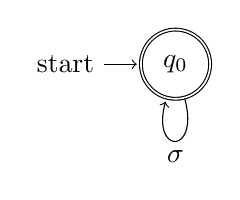
\begin{tikzpicture}[shorten >=1pt,node distance=3cm,on grid,auto] 
  			\node[state,initial, accepting] (q_0)   {$q_0$}; 
    		\path[->] 
    			(q_0) edge [loop below] node {$\sigma$} (q_0);
		\end{tikzpicture}
		
		\item Where $\sigma$ = the transition functions listed above.
	\end{itemize}
	
	\item Given the PDA below, convert it to a CFG and give the derivation of $aaabbb$ \\
	We can form our transitions as follows: 
	\begin{itemize}
		\item $\delta$(0, e, e) $\rightarrow$ (1 ,$\$$)
		\item $\delta$(1, a, e) $\rightarrow$ (1, a)
		\item $\delta$(1, b, a) $\rightarrow$ (2, e)
		\item $\delta$(2, b, a) $\rightarrow$ (2, e)
		\item $\delta$(2, e, $\$$) $\rightarrow$ (3, e)
	\end{itemize}
	
	We can construct the CFG below:
	\begin{itemize}
		\item A$_{03}$ = aA$_{12}$b
		\item A$_{12}$ = aA$_{12}$b $|$ ab
	\end{itemize}
	Our string $aaabbb$ derivation is given below: \\
	A$_{03}$ $\rightarrow$ aA$_{12}$b $\rightarrow$ aaA$_{12}$bb $\rightarrow$ aaabbb
	
	
	\item Give a informal description of a Turing machine that decides the language L = $\{$ w $|$ w contains an equal number of 0s and 1s $\}$ \\ 
	
	Let M be a turing machine $<$M,w$>$ where: \\
		\tabto{1cm}m = "on input w\\
			\tabto{2cm}1. Determine if W is a member of 0$^*$1$^*$. Reject if not.\\
			\tabto{2cm}2. Sweep from left to right and cross off 2 uncrossed positions. Accept if 0\\ 			   \tabto{2cm}or two positions were crossed off. Reject if only one position was crossed \tabto{2cm}off."\\
			This turing machine accepts L.
			
	\item Give a informal description of a Turing machine that decides the language L = $\{$ w $|$ w contains twice as many 0s as 1s $\}$ \\ 
	
	Let M be a turing machine $<$M,w$>$ where: \\
		\tabto{1cm}m = "on input w\\
			\tabto{2cm}1. Determine if W is a member of 0$^*$1$^*$. Reject if not.\\
			\tabto{2cm}2. Sweep from left to right and cross off a single 0 and two 1s. If you \tabto{2cm}cannot cross off exactly a single 0 and two 1s and no other elements are \tabto{2cm}uncrossed, then accept. Otherwise, reject." \\
			This turing machine accepts L.
	
	\item Show that the collection of decidable languages is closed under the operation of
complementation. \\

	Let M be a turing machine of a decidable language L. Let R be a turing machine that decides the complement of L. \\
	
	\tabto{1cm}Define R s.t. where: "On input w \\
		\tabto{2cm}1. Run M on w. If it accepts, reject. \\
		\tabto{2cm}2. Otherwise, accept." \\
	
	This turing machine shows that a decidable language is closed under complementation.
	\pagebreak
	\item Let INFINITE$_{DFA}$ = $\{$ $<$ A $>$ $|$ A is a DFA and L(A) is an infinite language $\}$. Show that INFINITE$_{DFA}$ is decidable. \\ 
	
	\tabto{1cm}Let M be a turing machine s.t. M = "On input $<A>$ where A is a DFA: \\
	\tabto{2cm}1. Let p be the number of states in A. \\
	\tabto{2cm}2. Construct a DFA D that accepts all strings of length k or more (meaning 		\tabto{2cm}there must be some loop). \\
	\tabto{2cm}3. Construct a DFA Z s.t. L(Z) = L(A) $\cap$ L(D). \\
	\tabto{2cm}4. Test whether L(B) = $\emptyset$ using E$_{DFA}$ T proved in class. \\
	\tabto{2cm}5. If T accepts, reject. If T rejects, accept. \\ 
	
	This turing machine shows that INFINITE$_{DFA}$ is decidable.
	
	\item Let T = $\{$ $<$ w $>$ $|$ M is a TM that accepts w$^r$ whenever it accepts w $\}$. Show that T is undecidable. \\ 
	
	\tabto{1cm}Let R decide T. Construct a TM S s.t. S = "On input $<M,w>$ \\
		\tabto{2cm}1. Create a TM Q s.t Q = "On input x\\
			\tabto{3cm}1. If x does not have the form 01 or 10, reject\\
			\tabto{3cm}2. If x has the form 01, accept\\
			\tabto{3cm}3. Else run w on M and accept if M accepts"\\
		\tabto{2cm}2. Run R on Q.\\
		\tabto{2cm}3. Accepts if R accepts, reject if R rejects." \\
	
	Since S decides A$_{TM}$ (since we have reduced it to this) which we have proven to be undecidable, we know that T is undecidable.
\end{enumerate}

\end{document}